% Test slide for temperature effects chart
\documentclass[8pt,aspectratio=169]{beamer}
\usetheme{Madrid}
\usepackage{graphicx}

% Color definitions
\definecolor{mlpurple}{RGB}{51,51,178}
\definecolor{mllavender3}{RGB}{204,204,235}

% Apply colors
\setbeamercolor{frametitle}{fg=mlpurple,bg=mllavender3}

\begin{document}

\begin{frame}[t]{Temperature Sampling: Control Randomness}
\vspace{-0.3cm}
\begin{center}
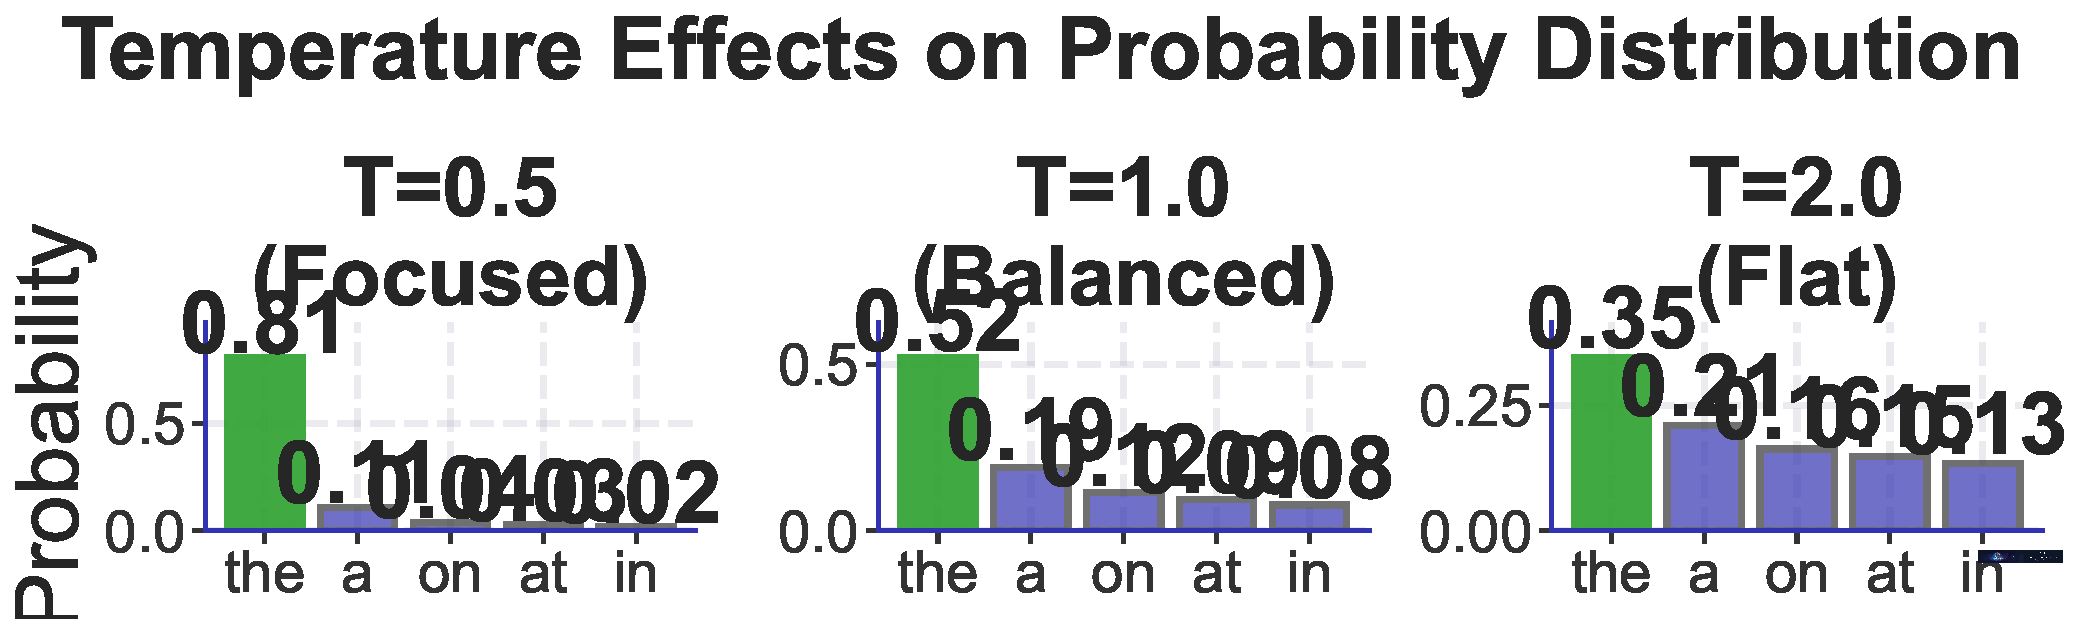
\includegraphics[width=0.65\textwidth]{../figures/temperature_effects_bsc.pdf}
\end{center}
\begin{center}
\textbf{Key Insight}: Temperature reshapes probability distribution
\end{center}
\end{frame}

\end{document}
